\section{Problem Statement}
\label{sec:problemStatement}

TEEs have had a transformational impact on the landscape of secure computing. They eliminate the operating system (OS) from the trusted computing base (TCB), enabling very lightweight applications to be executed securely in an hostile environment. However, TEEs generally only provide secure computation on the processor cores and cannot easily communicate with the external devices. Many current applications would benefit from such an interaction, either enabling new use-cases with inputs from sensors or unlocking massive performance gains from accelerators. Current TEEs generally do not support such use cases because they rely on the attacker-controlled OS to facilitate communication to an external device. Thus, the OS is part of the TCB again, violating one of the primary reasons to use a TEE. 
These use cases are usually solved by employing one of the following three approaches: 
\begin{enumerate}
    \item Design a fully dedicated system.
    \item Rent a dedicated virtual machine and place trust in the hypervisor.
    \item Continue relying on the operating system.
\end{enumerate}
We believe none of these approaches to be satisfactory due to cost and the need to trust codebases with millions of lines of code~\cite{torvalds2020linux,barham2003xen}.


\myparagraph{Use case scenario 1} While using the online banking system, the user must ensure that the banking application has exclusive access to her IO devices. This is a typical scenario of a trusted path between the user's IO peripherals and the trusted application (e.g., an enclave running on the CPU cores).

\emph{Challenge 1:} The trusted path requires two security properties: i) the IO data is actually reaching from the peripheral to the intended enclave while keeping the integrity (and possibly confidentiality) preserved, and ii) no other enclaves or the OS have access to the peripheral at the same time (unlike ARM TrustZone). TEEs generally ensure secure computation \emph{only} on the processor cores and cannot easily communicate with external devices such as peripherals. TEEs usually rely on the OS for communication with the such. Hence, several existing security and safety-critical applications that involve external peripherals are not easily enabled by the existing TEEs. 

\myparagraph{Use case scenario 2} In a multi-tenant accelerator, the client running a workload must ensure that the execution is isolated from other execution and the workload is running on the specific GPU that she configured. 

\emph{Challenge 2:} Conventional TEEs does not support such security feature either. Works such as Graviton~\cite{volos2018graviton} provides a framework to run enclaves on the GPUs, but it is only geared towards a specific peripheral (GPU). Hence, retrofitting such a solution to support a wide-range of peripherals is non-trivial. 

\myparagraph{Use case scenario 3} When an industrial plant operator decides to actuate a piece of machinery based on a sensor reading, the operator must ensure that the sensor reading is coming from a certified sensor.

\emph{Challenge 3:} A remote verifier must be able to attest to all critical components (enclaves running on the processor core and firmware running on the peripherals) and the communication links between them, to assert whether it is configured properly. For instance, the attestation report certifies that only a particular application has exclusive access to a specific peripheral. In short, in contrast to traditional TEEs, a remote verifier can attest to not only the authenticity and integrity of the enclave, but also the peripheral firmware that the enclave is communicating with.

\myparagraph{Use case scenario 4} In all the aforementioned applications, the platform user must know if a peripheral that she is using is disconnected and reconnected. And in-between the detachment and reattachment events, the peripheral remains unchanged. 

\emph{Challenge 4:} An enclave must be able to detect if a peripheral device is plugged out or replaced. This is the dynamic counterpart to the attestation above. We call a processor-local enclave that is aware of the surrounding state \emph{platform aware}. In general, the full state of a system is too detailed to be processed every time it changes or to meaningfully assess whether it is safe for a remote stakeholder to provide its data. Therefore, concretely this last challenge requires defining what parts of the state (and state transitions) of a system are relevant to ensure isolation and integrity of the communication between enclaves and peripherals.


 \emph{Challenge 5:} All of the above challenges should be addressed without making any significant changes into existing platforms and low development overheads on the existing application, driver, and peripheral firmware developers.



 In summary, we identify the following challenges:





In this paper, we investigate Trusted Execution Environments spanning an entire platform which we call \emph{platform isolation environments} (\name{}). Before delving into it, however, it is important to define what extending a TEE to an entire platform means and what the desired requirements of such a system are. Some specific examples of \name{}s already exist with single static external components in the form of Intel SGX connected to the management engine for monotonic counters~\cite{matetic2017rote}, or ARM TrustZone based solutions for trusted path~\cite{VButton,SeCloak}. However, we consider systems that can extend to virtually any kind of peripherals, allowing for dynamic reconfiguration of the TCB.\moritz{Maybe say that PIEs must remain general} To narrow the scope even more, we consider a \name to be a combination of multiple TEEs on individual components, e.g., a TEE on the CPU~\cite{keystone} and one on the GPU~\cite{volos2018graviton}. A \name{} should provide similar guarantees as traditional TEEs and eventually pave the way secure computation on an entire platform. %\moritz{Not clear yet how current existing systems are differentiated from what we are doin!}

We identify three main challenges that need to be solved to realize a \name{}. First, enclaves on the processor must be able to securely communicate to peripherals in a way that is isolated from the attacker-controlled operating system. Moreover, the communication different enclaves are peripherals are isolated from each other (unlike ARM TrustZone).

Second, a remote verifier must be able to attest to all critical components (enclaves running on the processor core and firmware running on the peripherals) and the communication links between them, to assert whether it is configured properly. For instance, the attestation report certify that that only a particular application has exclusive access to a certain peripheral. In short, in contrast to traditional TEEs, a remote verifier can not only attest the authenticity and integrity of the enclave, but also that peripheral firmware that the enclave is communicating with.


And third, a \name{} must be aware of the state of its components, e.g., it must be able to detect if a peripheral device is plugged out or replaced. This is the dynamic counterpart to the attestation above. We call a processor-local enclave that is aware of the surrounding state \emph{platform aware}. In general, the full state of a system is too detailed to be processed every time it changes or to meaningfully assess whether it is safe for a remote stakeholder to provide its data. Therefore, concretely this last challenge requires defining what parts of the state (and state transitions) of a system are relevant to ensure isolation and integrity of a \name.  %Thus, we rely on the TEEs of the individual components to be aware of their own state and only consider their interactions.


In summary, we identify the following challenges:
\moritz{Challenge 4: support wide range of existing peripherals. Easily add new peripherals}
\moritz{Challenge 5: Maintain as much compatibility with existing drivers}

\begin{mylist}

  \item \textbf{Isolated communication:} An enclave is able to communicate with other entities on the platform while the communication channel is isolated from the attacker-controlled operating system. The communication channel should be efficient and should require minimal changes to the underlying TEEs.
  
  \item \textbf{Platform-wide attestation:} The state of the entire platform, that involves the enclaves, connected peripherals, the secure communication channel between them, and the communication configuration must be verifiable by a local and remote verifier. A platform-wide attestation also includes the authenticity and integrity of the firmware of the external peripherals. 

  \item \textbf{Platform awareness:} Any enclave must be aware of the state of the entire platform at all times. Upon any state-change, the enclave should have the possibility to react, e.g., it may want to halt its execution when the peripheral it is communicating gets replaced. %We call this: \emph{platform awareness}.

\end{mylist}







\subsection{System Model}
\label{sec:problemStatement:systemModel}

We consider modern platforms that typically consist of multiple interconnected hardware components. In practice, this usually involves the central processor, memory, and various peripherals such as storage devices, graphics cards, sensors, and in general I/O devices. These components are interconnected over various buses. In reality, hardware components might themselves contain multiple parts such as independent integrated systems. However, we ignore their inner architecture and consider them as a single logical unit with a predefined interface. In the rest of the paper, we will use \emph{processor} to indicate a central processing unit (CPU) and \emph{peripheral} for any other external component. Figure\ref{fig:bus} depicts an overview of the platform architecture with connected peripheral devices. Most peripherals are not purely controlled by application-specific integrated circuits (ASIC), but they are managed by a microcontroller that runs some software called \emph{firmware}. Depending on the peripheral, firmware can be of varying levels of complexity. For example, input devices such as keyboards usually only contain basic firmware. In contrast, the firmware of a data-center accelerator may be extremely complex. The processor also runs a vast software stack, from the BIOS to an operating system and user-space applications. 
%Any application can interact with a peripheral through the driver in the operating system.


% 
% \begin{figure}[t]
%   \centering
%   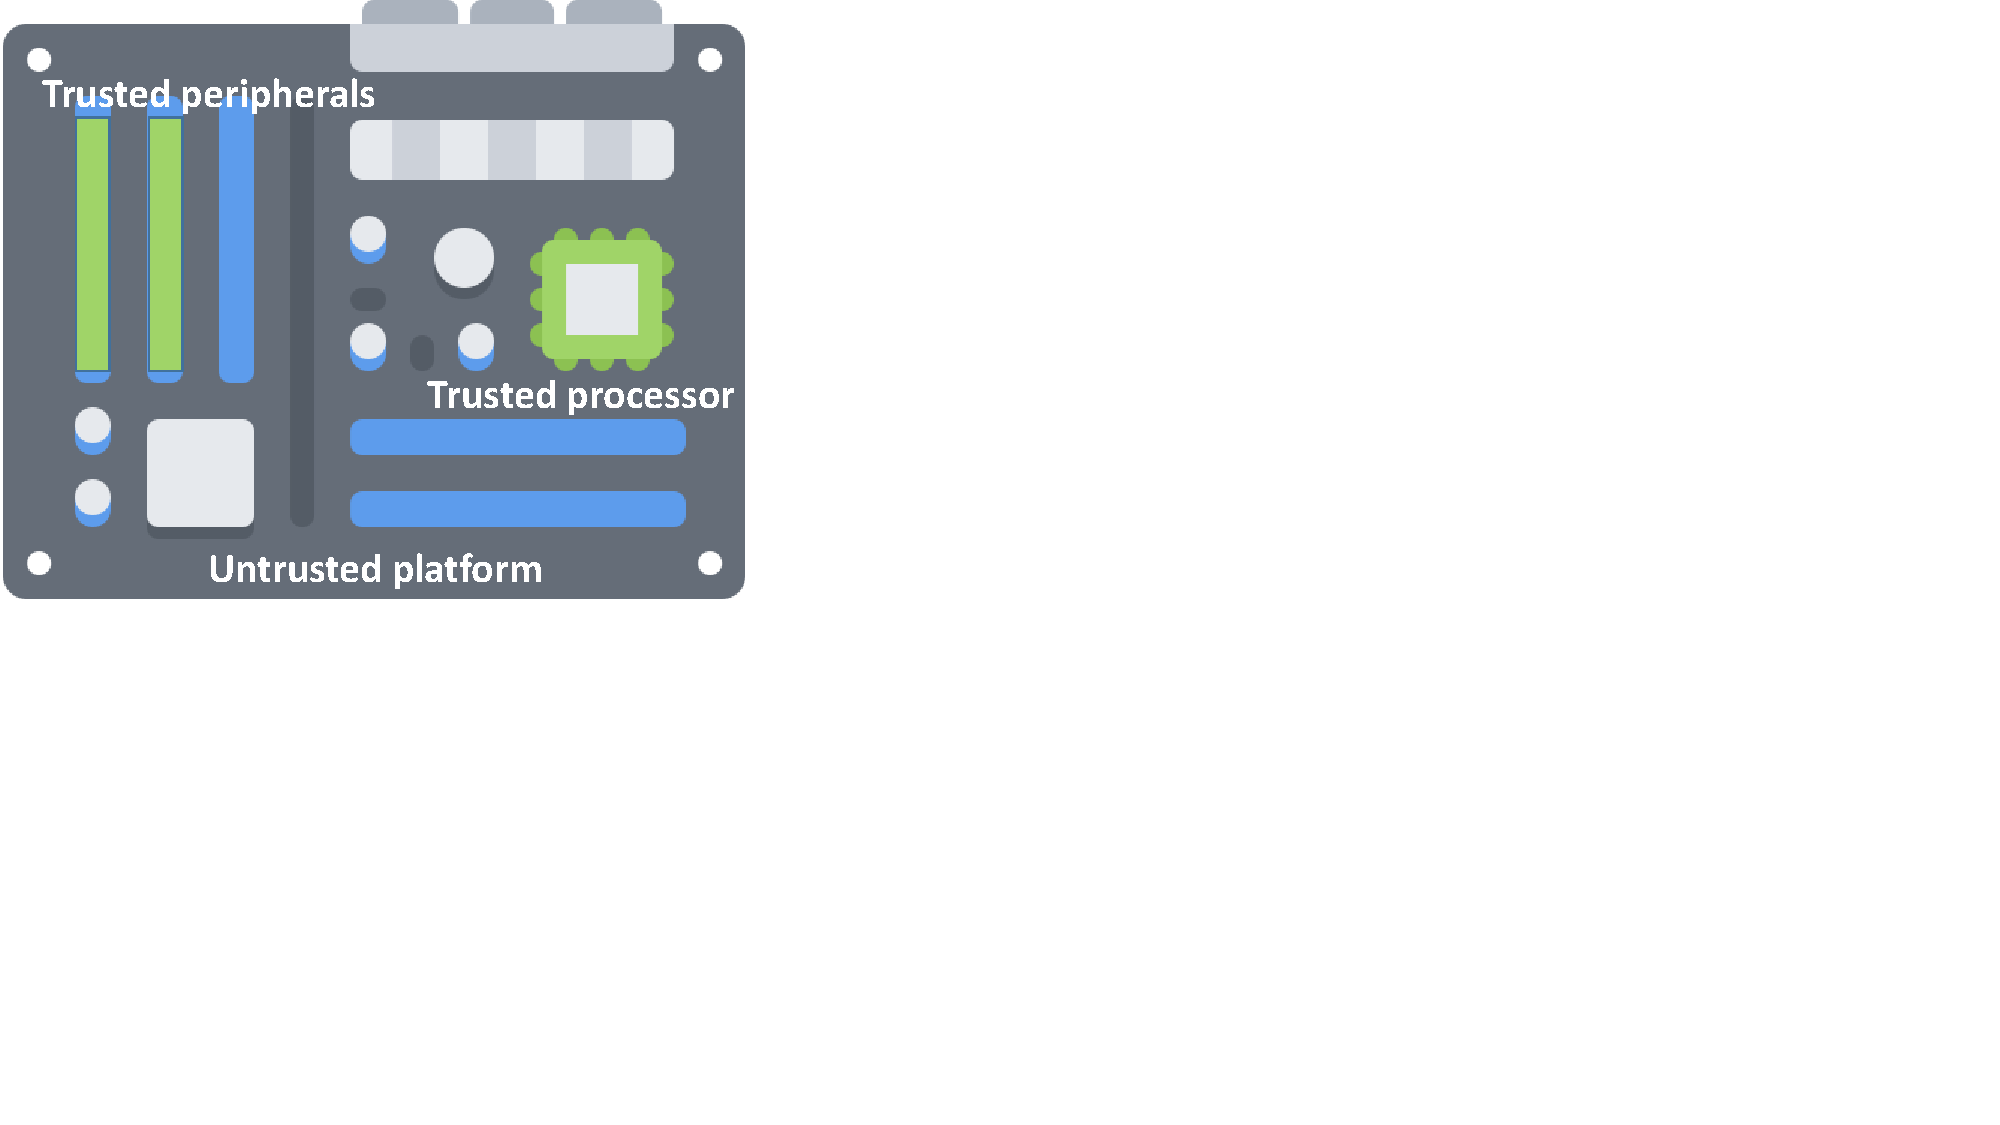
\includegraphics[trim={0 9cm 21cm 0}, clip, width=0.65\linewidth]{trustModel.pdf}
%   \caption{\textbf{Trust assumption.} The processor package and peripheral hardware are trusted. Rest - the interconnects, DRM, OS are untrusted.}
%   \label{fig:trustModel}
% \end{figure}

